\xchapter{Experimentos}{Coleta e análise de dados}

Nesta seção irei mostrar o resultado das medições de latência realizadas no Raspberry. Será comparado os valores entre diferentes versões do kernel, entre diferentes tipos de interrupção e entre diferentes cargas na CPU.

\section{Configuração do teste}

As medições foram agrupadas por tipo de kernel, tipo de interrupção e carga na CPU, resultando em um total de 18 grupos de teste. Cada grupo passou por uma bateria de medições. Em cada bateria de teste, foram executadas 50000 medições com um intervalo de 20ms entre elas. 

O INTSight gera 2 arquivos no format CSV para cada bateria de medições. Um dos arquivos chamado name contém o tipo de evento que disparou a coleta do tempo de sistema. Outro arquivo com o nome do tipo de contador utilizado, ktime\_mono\_fast em todos os teste deste trabalho, contém o valor do contador no instante que a coleta foi disparada. Em ambos os arquivos, cada medição ocupa uma linha do arquivo.

No repositório do INTSight é disponibilizado um script em R que faz o junção destes arquivos em um único utilzando as seguintes informação: position (posição do item dentro da medição), run (número da medição dentro da bateria), name (evento que disparou a medição), ktime\_mono\_fast (valor do contador de tempo). Para consolidar os resultados das 18 baterias, foi feito um script python que encontra-se disponível em github. Este script também faz um tratamento dos dados úteis, pois o INTSight pode apresentar valores zerados quando ocorre algum erro durante uma medição.

\section{Visão geral}

A primeira letra representa o kernel testado: (r)aspberry padrão ou (p)reempt-RT.
A segunda letra é o tipo de interrupção testado: (s)oftirq, (t)asklet, (w)orkqueue.
O terceiro caracter é a carga na cpu: 0 thread, 1 thread, (m)any threads (256).

Na tabela \ref{table:rpi} temos uma visão sumarizada do tempo de latência em nanossegundos de todos os testes realizados com o kernel padrão enquanto na tabela \ref{table:prt} temos uma visão dos testes no Preempt-RT.

\begin{table}[h!]
\centering
\begin{center}
\begin{tabular}{|c|r|r|r|r|r|r|r|r|r|}
\toprule
Percentil &    rs0 &     rs1 &    rsm &    rt0 &    rt1 &    rtm &    rw0 &     rw1 &      rwm \\
\midrule
    min &    833 &     782 &    781 &    625 &    938 &    573 &   7604 &    5730 &     5156 \\
    25\% &   1041 &     937 &    937 &   1145 &   1145 &   1146 &   8021 &    8073 &     8750 \\
    50\% &   1042 &     938 &    938 &   1146 &   1146 &   1146 &   8124 &    8177 &     8854 \\
    75\% &   1094 &     990 &    990 &   1198 &   1198 &   1250 &   8229 &    8802 &     8958 \\
    90\% &   1146 &    1042 &   1042 &   1302 &   1302 &   1406 &   8489 &    9011 &     9218 \\
    95\% &   1198 &    1823 &   1146 &   1406 &   1927 &   2187 &  11823 &    9896 &     9791 \\
    99\% &   6041 &    5833 &   5937 &   6250 &   6251 &   6198 &  16667 &   18021 &    18282 \\
    max &  15156 &  191821 &  19375 &  34998 &  25834 &  45260 &  84635 &  983798 &  4153458 \\
\bottomrule
\end{tabular}
\end{center}
\caption{Principais dados das medidas do kernel padrão}
\label{table:rpi}
\end{table}

\begin{table}[h!]
\centering
\begin{center}
\begin{tabular}{|c|r|r|r|r|r|r|r|r|r|}
\toprule
Percentil &    ps0 &    ps1 &    psm &    pt0 &    pt1 &    ptm &    pw0 &     pw1 &    pwm \\
\midrule
    min &   1197 &   1146 &   1197 &   1614 &   1563 &   1614 &  11563 &   11562 &  11562 \\
    25\% &   1406 &   1406 &   1406 &   1823 &   1823 &   1823 &  12084 &   12084 &  12083 \\
    50\% &   1407 &   1407 &   1458 &   1875 &   1875 &   1875 &  12239 &   12240 &  12187 \\
    75\% &   1459 &   1458 &   1459 &   1927 &   1927 &   1875 &  12396 &   12447 &  12344 \\
    90\% &   1510 &   1510 &   1510 &   1980 &   1979 &   1927 &  12761 &   12760 &  12656 \\
    95\% &   1511 &   1511 &   1511 &   2032 &   2031 &   1979 &  13334 &   13177 &  13073 \\
    99\% &   1979 &   1823 &   1979 &   2448 &   3073 &   3125 &  21615 &   23490 &  19323 \\
    max &  18698 &  17656 &  17657 &  17343 &  16979 &  17865 &  80526 &  259583 &  86198 \\
\bottomrule
\end{tabular}
\end{center}
\caption{Principais dados das medidas do Preempt-RT}
\label{table:prt}
\end{table}

% \begin{figure}
%     \centering
%     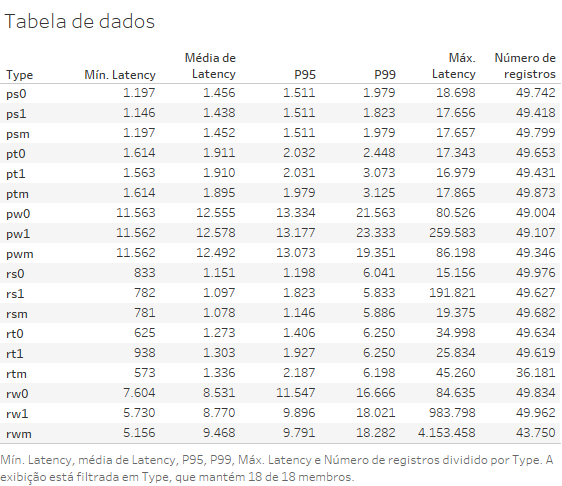
\includegraphics{graficos/Tabeladedados.png}
%     \caption{Medições de latência}
%     \label{tableau}
% \end{figure}

% \subsection{Divisão por tipo de kernel}

% \begin{itemize}
% \item Normal
% \item Preempt-RT
% % \item Xenomai
% \end{itemize}

% \subsection{Divisão por irqs}

% \begin{itemize}
% \item Softirq
% \item Tasklet
% \item Workqueue
% \end{itemize}

% \subsection{Divisão por carga na cpu}

% \begin{itemize}
% \item Ociosa
% \item Um processo
% \item Sobrecarga (256 processos)
% \end{itemize}

% \section{Expectativas}

% Preempt-RT mais lento na médio, melhor pior caso, menos variação.

\section{Resultados}

\subsection{Comparativo entre kernel}

\subsubsection{Softirq sem carga}

\begin{figure}[H]
  \centering
  \begin{minipage}[b]{0.4\textwidth}
    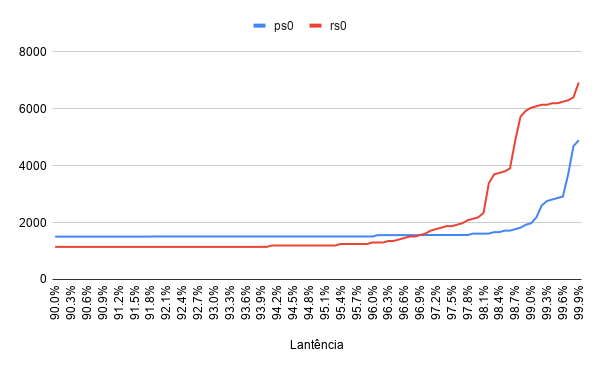
\includegraphics[width=\textwidth]{graficos/ps0-rs0.png}
    \caption{PS0 x RS0}
    \label{tableau}
  \end{minipage}
  \hfill
  \begin{minipage}[b]{0.4\textwidth}
    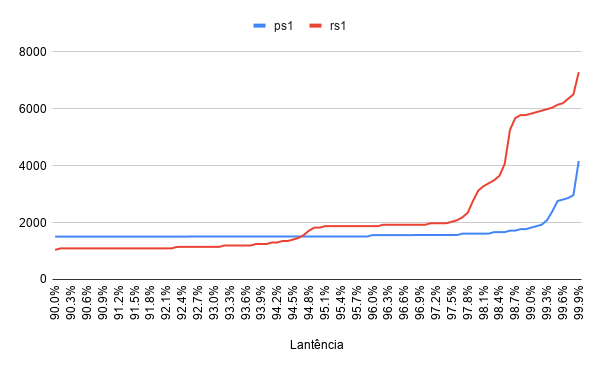
\includegraphics[width=\textwidth]{graficos/ps1-rs1.png}
    \caption{PS1 x RS1}
    \label{tableau}
  \end{minipage}
\end{figure}


\subsection{Comparativo por tipo de interrupção}
\subsection{Comparativo por carga de trabalho}